\section{Motivation} \label{sec:motivation}

This section motivates for a more powerful function-merging technique with
examples that highlight some of the weaknesses of the existing solutions, while
also demonstrating how our optimization is able to overcome them.
These examples contain real functions\footnote{We have changed very lightly some
of the names used in the functions so that the code fits nicely in the paper.},
extracted from the SPEC CPU2006 benchmark suite, that were carefully selected to
show two distinct scenarios.
The proposed optimization is the \textit{first} technique able to merge the
functions shown in these examples.
Note that, although we present the examples at the source level, the
optimizations are actually implemented at the IR level.

\begin{figure}[th]
  \centering
  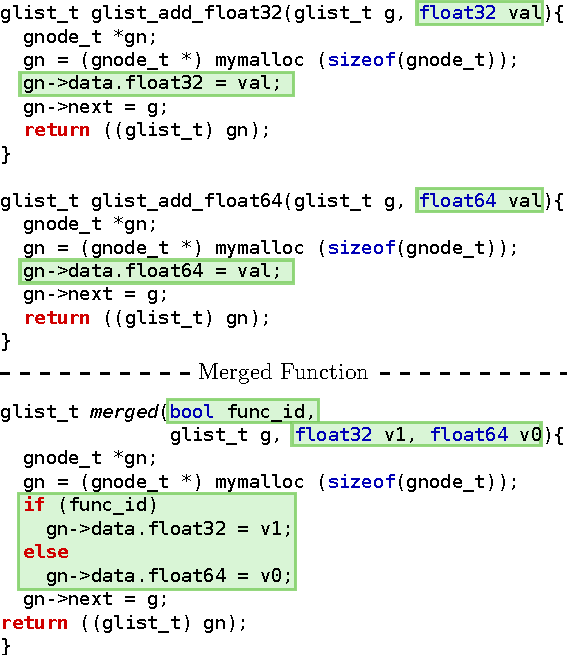
\includegraphics[width=.95\linewidth]{figs/sphinx-example.pdf}
  \caption{Functions with different list of parameters.}
  \label{fig:sphinx-example}
\end{figure}

Figure~\ref{fig:sphinx-example} shows two complete functions extracted from the
\text{482.sphinx3} benchmark.
Although these two functions seem identical, they operate on parameters of
different types, namely, \textit{float32} and \textit{float64}.
We highlight the segments where the functions differ from each other.
As we have described in Section~\ref{sec:background}, all the existing 
function-merging techniques require that both functions have exactly the same 
list of parameters, with the same types and the same order.
Moreover, this also means that the two functions contain instructions with
different types.
As a result, no one of the existing techniques would be able to merge these two
nearly identical functions.
However, the proposed optimization is able to merge them as shown at the bottom
of Figure~\ref{fig:sphinx-example}.
First, we merge both lists of parameters, adding an extra parameter used as an
identifier to distinguish between the functions.
Then, we guard the execution of the instructions that are unique to one of
the functions using the function identifier.

\begin{figure}[th]
  \centering
  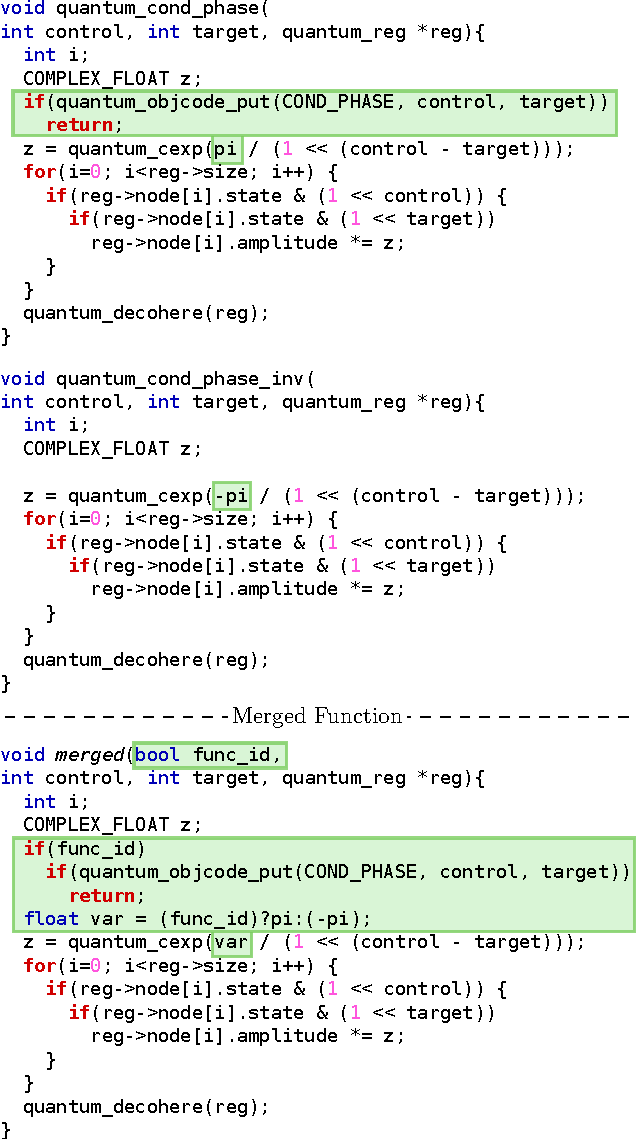
\includegraphics[width=\linewidth]{figs/libquantum-example.pdf}
  \caption{Functions with different CFGs.}
  \label{fig:libquantum-example}
\end{figure}

Figure~\ref{fig:libquantum-example} shows two complete functions extracted from
the \text{462.libquantum} benchmark.
Although these two functions have the same signature, i.e., the same return type
and list of parameters, they differ in some parts, including their CFGs.
The existing techniques are unable to merge them due mainly to the structural
differences in their CFGs, as we have described in Section~\ref{sec:background}. 
Similar to the previous example, the proposed optimization is also able to merge
these two functions, as shown at the bottom of Figure~\ref{fig:libquantum-example}.
Basically, we guard the execution of the code that are unique to one of the
functions using the function identifier added to the list of parameters.

